Dieser Anhang ist ein \texttt{Jupyter Notebook}. Hier wird eine mögliche
Implementation des präsentierten Algorithmus vorgeführt. Der Quellcode
wurde in \texttt{Python 3.7.9} geschrieben und ausgeführt.

Im nächsten Block werden die notwendigen Pakete importiert.

\begin{lstlisting}[language=Python]
import numpy as np
import pandas as pd
import matplotlib
import matplotlib.pyplot as plt
import scipy as sp
from scipy.fft import ifft
from scipy.fft import fft
from scipy.interpolate import interp1d
from scipy.optimize import minimize

# matplotlib figure config
matplotlib.rcParams['figure.dpi'] = 1000
matplotlib.rcParams["figure.figsize"] = (6.299213, 3.149606) # 16cm by 8cm
matplotlib.rcParams["font.family"] = "Minion Pro Regular"
matplotlib.rcParams["text.usetex"] = True
matplotlib.rcParams['font.size'] = 11
%config InlineBackend.figure_formats = ["png"]
\end{lstlisting}

\hypertarget{rauschformungsfilter}{%
\subsection{Rauschformungsfilter}\label{rauschformungsfilter}}

Der Filter wird als FIR Filter anhand von ISO226 konstruiert. Der Ablauf
besteht wie folgt:

\begin{enumerate}
\tightlist
\item
  ISO226 Frequenzverlauf für 0 Phon erstellen
\item
  Frequenzverlauf auf das gesamte Spektrum (bis \(\frac{f_s}{2}\))
  extrapolieren
\item
  Wertemenge der Extrapolation limitieren
\item
  Verstärkung und Reduktion über das Spektrum numerisch bestimmen und
  auf 0 optimieren
\item
  FIR Kernel durch Inverse-Fourier Transformation bestimmen
\item
  Kernel durch Fenster fertigstellen
\end{enumerate}

\hypertarget{psychoakustische-zielfunktion-nach-iso-erstellen}{%
\subsubsection{Psychoakustische Zielfunktion nach ISO
erstellen}\label{psychoakustische-zielfunktion-nach-iso-erstellen}}

Diese Implementation ist dem Standard entnommen und lediglich nach
\texttt{Python} konvertiert.

\begin{lstlisting}[language=Python]
# adapted from Jeff Tackett
# https://www.mathworks.com/matlabcentral/fileexchange/7028-iso-226-equal-loudness-level-contour-signal
def ISO226(phon):
    f = np.array([20, 25, 31.5, 40, 50, 63, 80, 100, 125, 160, 200, 250, 315, 400, 500, 630, 800, 1000, 1250, 1600, 2000, 2500, 3150, 4000, 5000, 6300, 8000, 10000, 12500])
    af = np.array([0.532, 0.506, 0.480, 0.455, 0.432, 0.409, 0.387, 0.367, 0.349, 0.330, 0.315, 0.301, 0.288, 0.276, 0.267, 0.259, 0.253, 0.250, 0.246, 0.244, 0.243, 0.243, 0.243, 0.242, 0.242, 0.245, 0.254, 0.271, 0.301])
    Lu = np.array([-31.6, -27.2, -23.0, -19.1, -15.9, -13.0, -10.3, -8.1, -6.2, -4.5, -3.1, -2.0, -1.1, -0.4, 0.0, 0.3, 0.5, 0.0, -2.7, -4.1, -1.0, 1.7, 2.5, 1.2, -2.1, -7.1, -11.2, -10.7, -3.1])
    Tf = np.array([78.5, 68.7, 59.5, 51.1, 44.0, 37.5, 31.5, 26.5, 22.1, 17.9, 14.4, 11.4, 8.6, 6.2, 4.4, 3.0, 2.2, 2.4, 3.5, 1.7, -1.3, -4.2, -6.0, -5.4, -1.5, 6.0, 12.6, 13.9, 12.3])

    if((phon < 0) | (phon > 90)):
        return Lp, f
    else:
        Ln = phon

        # SPL from loudness level (iso226 sect 4.1)
        Af = 4.47E-3 * (pow(10, (0.025*Ln)) - 1.15) + \
            pow((0.4 * pow(10, (((Tf+Lu)/10)-9))), af)

        Lp = ((10./af) * np.log10(Af)) - Lu + 94

        return Lp, f

spl, f = ISO226(0) # evaluate at 0 Phon
\end{lstlisting}

\hypertarget{extrapolieren}{%
\subsubsection{Extrapolieren}\label{extrapolieren}}

\begin{lstlisting}[language=Python]
FS = 48000
LINE_SAMPLES = 1024

# resample and interpolate curve as spline
newF = np.linspace(0, FS//2, LINE_SAMPLES)
spline = interp1d(f, spl, kind="cubic", fill_value="extrapolate", bounds_error=False)
spline_interp = spline(newF)
\end{lstlisting}

\hypertarget{wertemenge-begrenzen}{%
\subsubsection{Wertemenge begrenzen}\label{wertemenge-begrenzen}}

\begin{lstlisting}[language=Python]
# soft-clamp
MAX_EXCURSION_HIGH = 20
spline_clamped = np.tanh((spline_interp/MAX_EXCURSION_HIGH)) * MAX_EXCURSION_HIGH

# hard-clamp
spline_clamped = (spline_clamped / np.max(np.abs(spline_clamped)))
\end{lstlisting}

\hypertarget{verstuxe4rkung-optimieren}{%
\subsubsection{Verstärkung optimieren}\label{verstuxe4rkung-optimieren}}

Der Fehler wird berechnet mit: \[
E(g) = \left( \frac{1}{N} \sum_{i=0}^{N} s[i] + g \right)^2
\] wobei \(s[i]\) die diskreten Werte der modifizierten Zielfunktion
sind.

\begin{lstlisting}[language=Python]
def integrate(g, *args):
    # square of numeric integral
    return np.power( (1/len(args[0])) * np.sum(args[0] + g) , 2)

# optimize spline gain (y offset) to achieve equal amplification and attenuation
# sum of all (shaped) noise must be 0 or greater (not negative, since energy musnt be lost)
optimized_gain_average = sp.optimize.minimize(
    fun=integrate, x0=[0], args=(spline_clamped), method='Powell', tol=1e-16, options={'disp': False})

# apply optimized gain
OPTIMIZED_GAIN = optimized_gain_average.x[0]
optimized_spline = (spline_clamped + OPTIMIZED_GAIN)
\end{lstlisting}

\hypertarget{fir-kernel-erstellen}{%
\subsubsection{FIR Kernel erstellen}\label{fir-kernel-erstellen}}

Aufgrund der Implementation der \texttt{FFT} bzw der \texttt{IFFT}
Funktion muss die Ausgabe noch bearbeitet werden. Imaginäre Frequenzen
sind nur für die Transformation notwendig.

\begin{lstlisting}[language=Python]
# interpolate and evaluate
spline_zero = np.append(optimized_spline[0], optimized_spline)
omega = np.linspace(0, np.pi, len(spline_zero))
Hd = interp1d(omega, spline_zero, kind="cubic", fill_value="extrapolate", bounds_error=False)

N = 512 # N Taps to calculate
k = np.linspace(0, N-1, N)
Hk = Hd( (2 * np.pi * k )/N )

if N % 2 == 0:
    UL = (N//2) - 1 # even
else:
    UL = (N-1) // 2 # odd

# perform inverse fft and scale
h = np.real(ifft(Hk))
h = h / np.max(np.abs(h))
h = h * (2 / (np.pi))

# shift fft to generate FIR kernel
left = h[UL:]
right = h[:UL]
kernel = np.append(left, right)
\end{lstlisting}

\hypertarget{fensterfunktion}{%
\subsubsection{Fensterfunktion}\label{fensterfunktion}}

Die Fensterfunktion ist hier ein einfaches Kosinusfenster der Form:
\[w[n] = \frac{\cos \left( \frac{2\pi n}{N}-\pi \right)}{2} + \frac{1}{2} \qquad \forall n \neq 0\]
wobei \(N\) die Anzahl der \gls{fir} Filter Taps ist.

\begin{lstlisting}[language=Python]
TAPS = len(kernel) # taps could be less than the generated kernel
tap_xspace = np.linspace(0, TAPS + 1, TAPS)

window = np.cos(np.linspace(-np.pi, np.pi, TAPS)) / 2 + 0.5
kernel = kernel * window

fig, axs = plt.subplots(1, 2)
axs[0].plot(tap_xspace, window, color="#f18700", lw=1)
markerline, stemlines, baseline = axs[0].stem(kernel, markerfmt=".")
plt.setp(markerline, 'color', "#13a538")
plt.setp(stemlines, 'color', "#13a538")
plt.setp(stemlines, 'linewidth', 0.5)

axs[1].plot(tap_xspace, window, color="#f18700", lw=1)
markerline, stemlines, baseline = axs[1].stem(kernel, markerfmt=".")
plt.setp(markerline, 'color', "#13a538")
plt.setp(stemlines, 'color', "#13a538")
plt.setp(stemlines, 'linewidth', 0.5)
axs[1].set_xlim([TAPS//2 -18, TAPS//2 + 20])

plt.show()
\end{lstlisting}

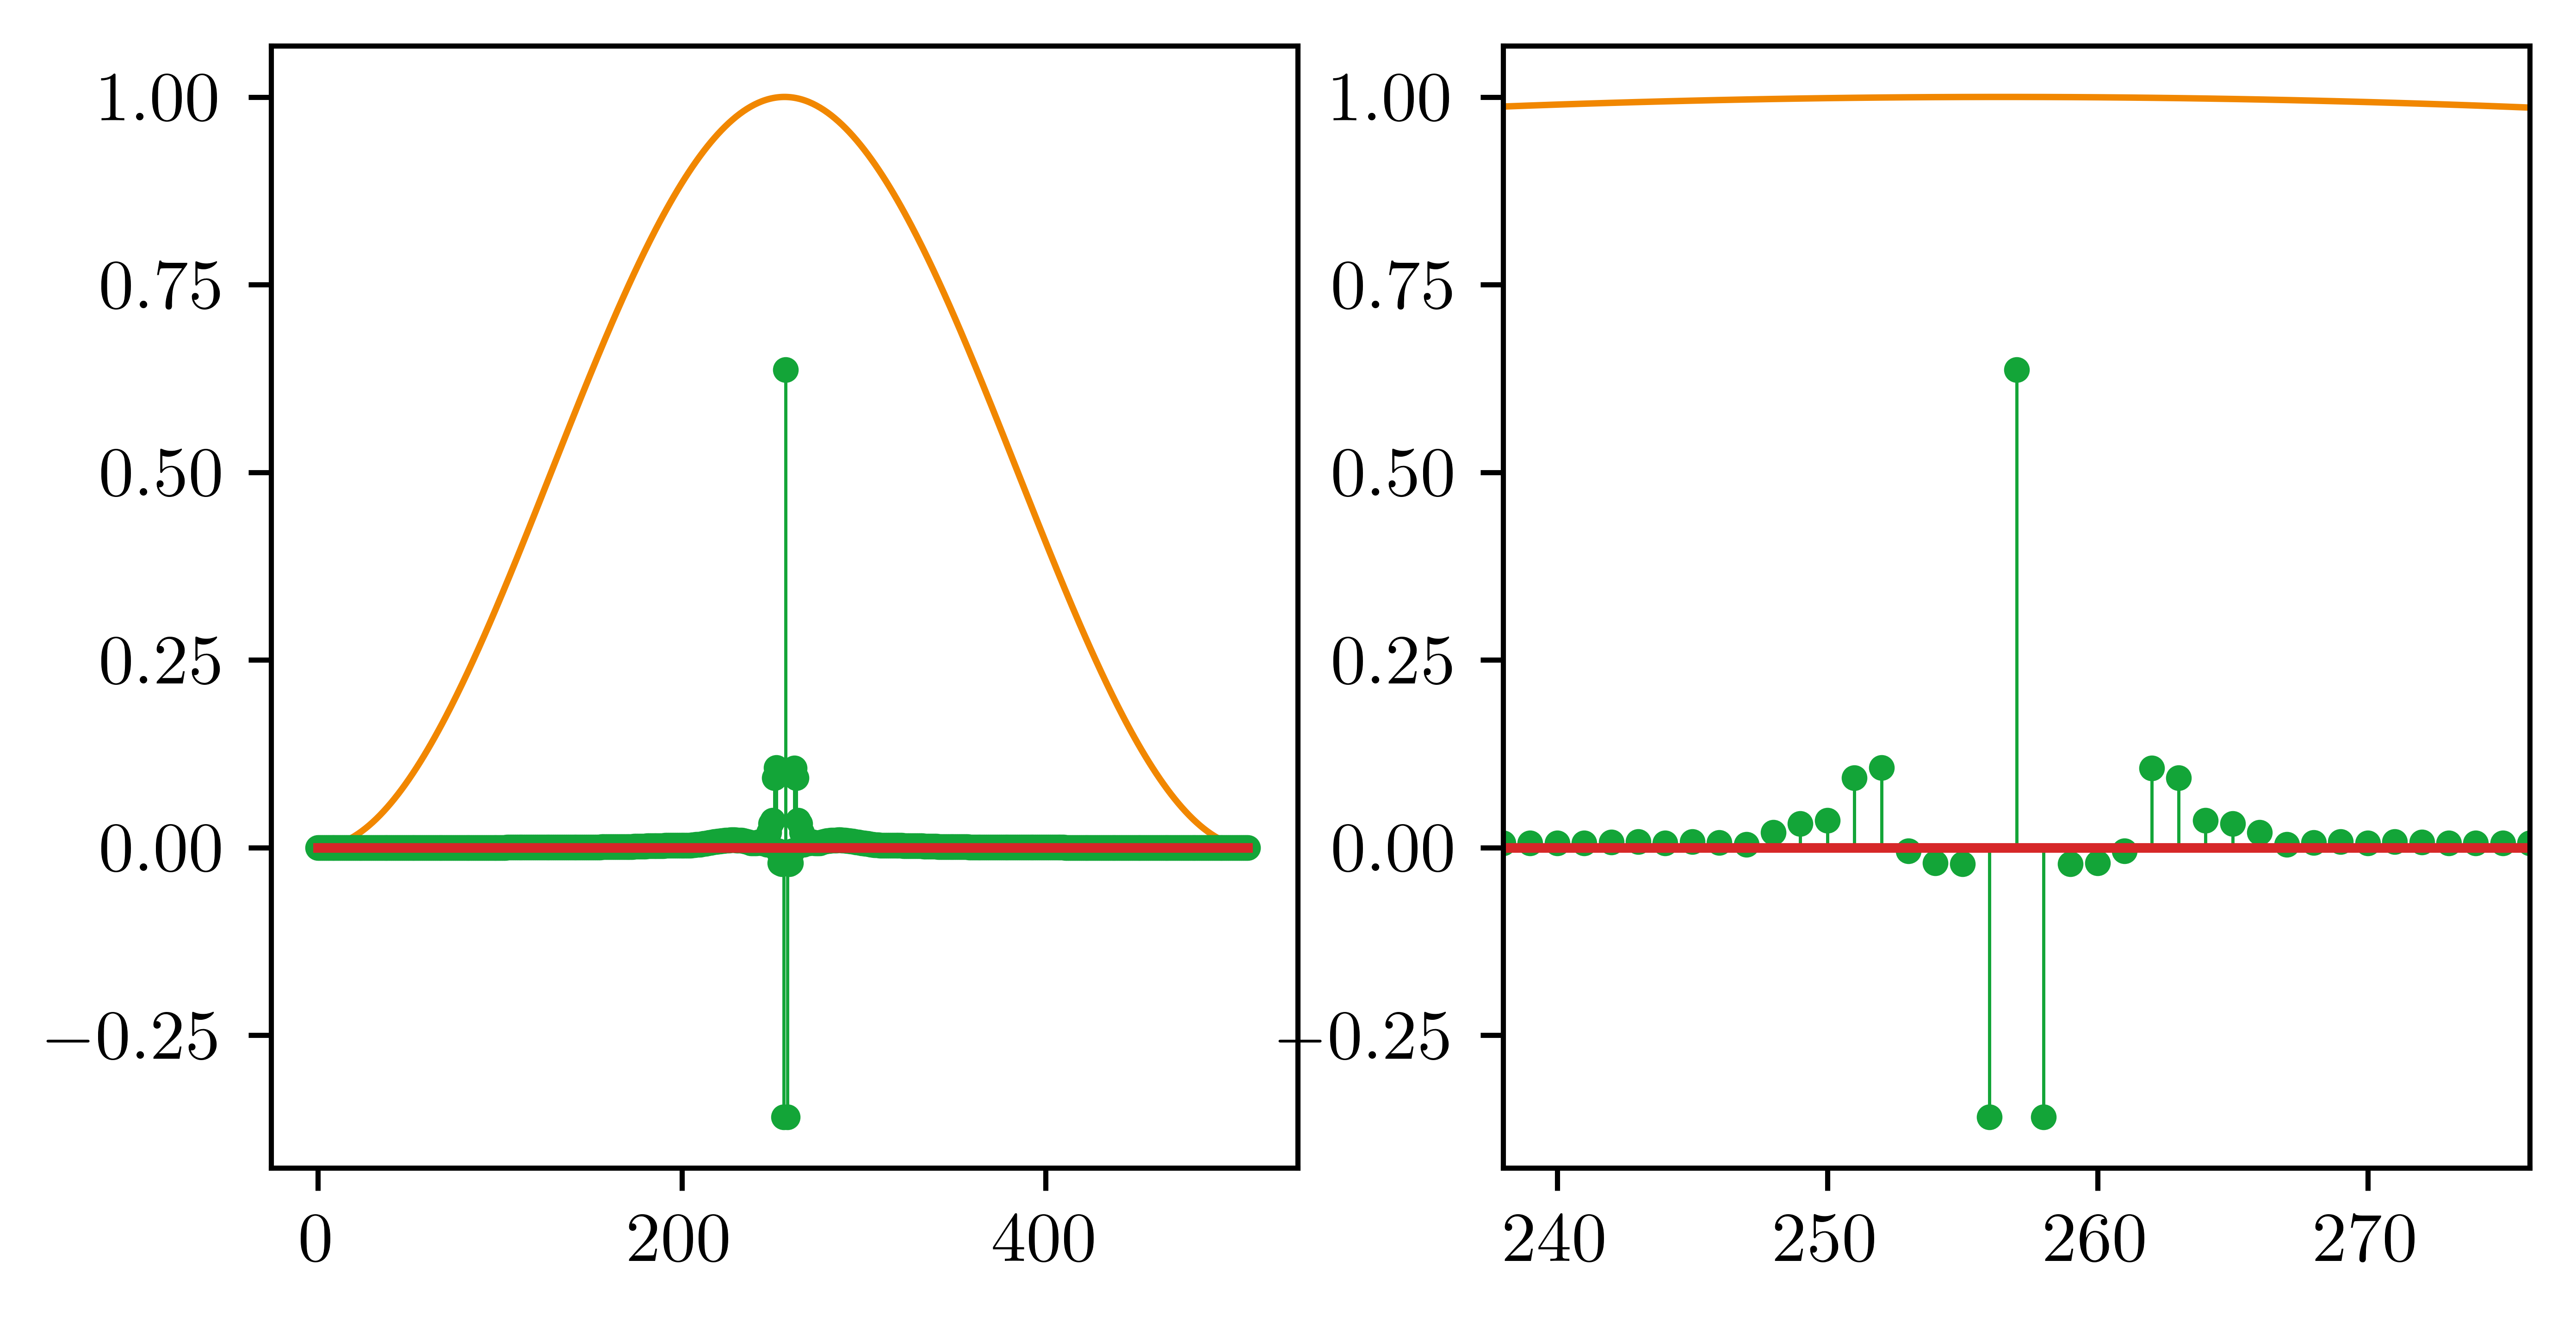
\includegraphics{./img/242aea9dbf6c58987e03c8555202b017345941e0.png}

Die grünen Punkte repräsentieren die individuellen \gls{fir} Taps. Die
rote Linie ist die Baseline um 0 zur Referenz. Das Fenster wird durch
den orangen Plot gezeichnet. Der linke Plot zeigt alle Taps, der rechte
zeigt nur einen Ausschnitt um die Mitte zentriert.

Wie zu erwarten sind die Taps, wie bei einem \gls{fir} Filter zu
erwarten, um \(\frac{\texttt{N}}{2}\) zentriert. Anders als der
standardmäßige \(\text{sinc} (x)\) Filter ist die maximale Amplitude
jedoch \(<1\).

\hypertarget{demonstration-des-filters}{%
\subsection{Demonstration des Filters}\label{demonstration-des-filters}}

Um zu demonstrieren, dass der konstruierte Filter funktioniert, wird ein
anschauliches Beispiel geliefert. Ein Signal wird in hoher Bit-Tiefe
erstellt. Dieses wird folgend stark quantisiert. Eine weitere Version
dieses Signals wird mit subtraktivem \gls{tpdf} Dither versehen.
Anschließend wird eine weitere Kopie durch den erstellten Filter
geformt.

\hypertarget{testsignal}{%
\subsubsection{Testsignal}\label{testsignal}}

Im Folgenden wird ein einfaches Testsignal erstellt. Dieses ist ein
Sinus mit \(f=100\) Hertz bei einer Abtastrate \(f_s\) von 48 Kilohertz
über eine Sekunde. Das Signal hat die allgemeine Form von
\[s(t) = \sin (2 \pi f t)\]

\begin{lstlisting}[language=Python]
FS = 48000
frequency = 100
duration = 1
t = np.linspace(0, duration, FS * duration)
signal = np.sin(frequency * 2 * np.pi * t)
\end{lstlisting}

Anschließend wird die Fourier Transformation des Signals gezeigt. Darin
ist ein klarer Hochpunkt bei \(10^2\) Hertz zu erkennen. Im Bereich
darüber bis hin zur halben Abtastfrequenz befinden sich
Konvertierungsartefakte, welche zu diesem Zeitpunkt ignoriert werden
können.

\begin{lstlisting}[language=Python]
bits = 15 # 15 bits scale due to sign bit
scale = 2**(bits-1) # -1 for a bit headroom in anticipation of dither
signal_scaled = (scale * signal).astype(np.int16)

plt.plot(np.abs(fft(signal_scaled)[1:FS//2]), color="#0085c8", lw=1)
plt.grid(which="both", linewidth=0.2)
plt.loglog()
plt.xlabel("$f$ in Hz")
ylim=plt.gca().get_ylim()
plt.show()
\end{lstlisting}

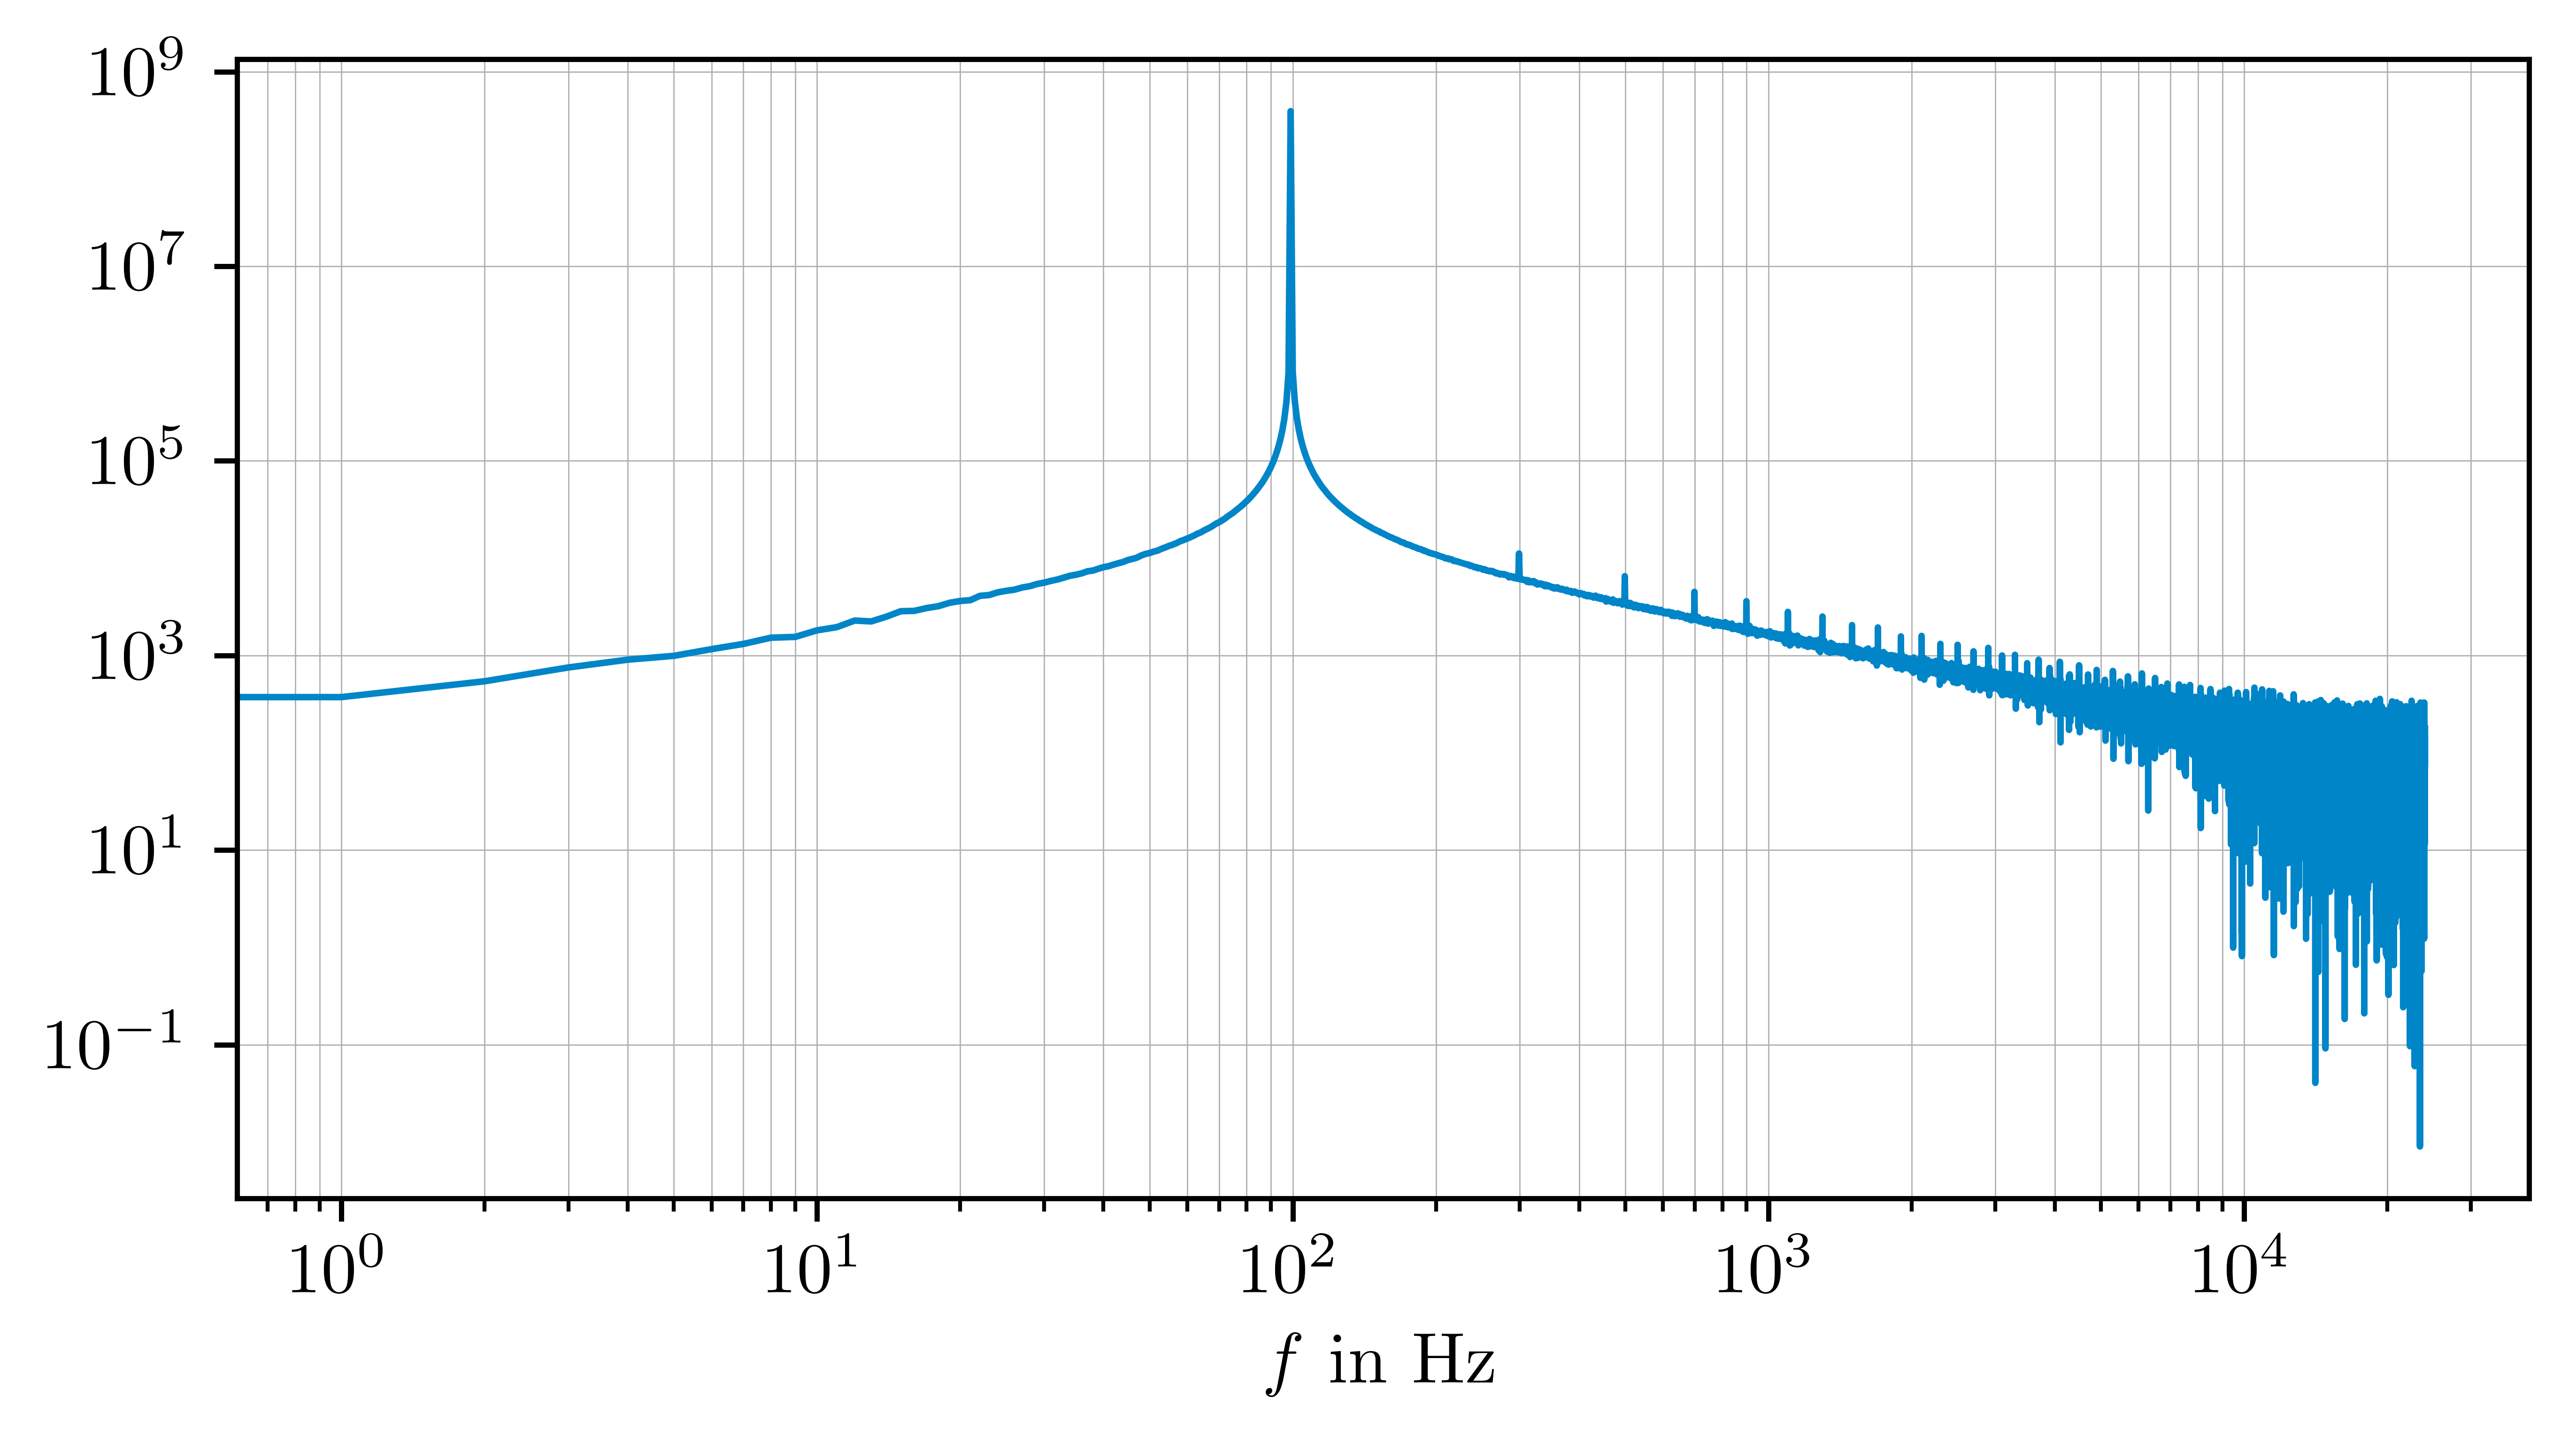
\includegraphics{./img/de9c4c704937869e21407a577db0ca1c99eb2ed8.png}

\hypertarget{dither}{%
\subsubsection{Dither}\label{dither}}

\begin{lstlisting}[language=Python]
# TPDF dither using two uncorellated noise sources
dither = np.random.rand(len(signal)) + np.random.rand(len(signal))
dither_scaled = (dither * (2**8)).astype(np.int16) # scale dither (usually only to 1 LSB)

fig, axs = plt.subplots(1, 2)
axs[0].hist(dither, facecolor="#17a2b0", lw=1, ec="w")
axs[0].plot([0, FS/5, 0], color="#f18700", linestyle="dashed")
axs[0].set_title("Dither histogram")
plt.xlabel("value")

axs[1].plot(np.abs(fft(dither)[1:FS//2]), color="#17a2b0", lw=1)
axs[1].grid(which="both", linewidth=0.2)
axs[1].loglog()
axs[1].set_ylim(ylim)
axs[1].set_title("Dither spectrum")
plt.xlabel("$f$ in Hz")

plt.show()
\end{lstlisting}

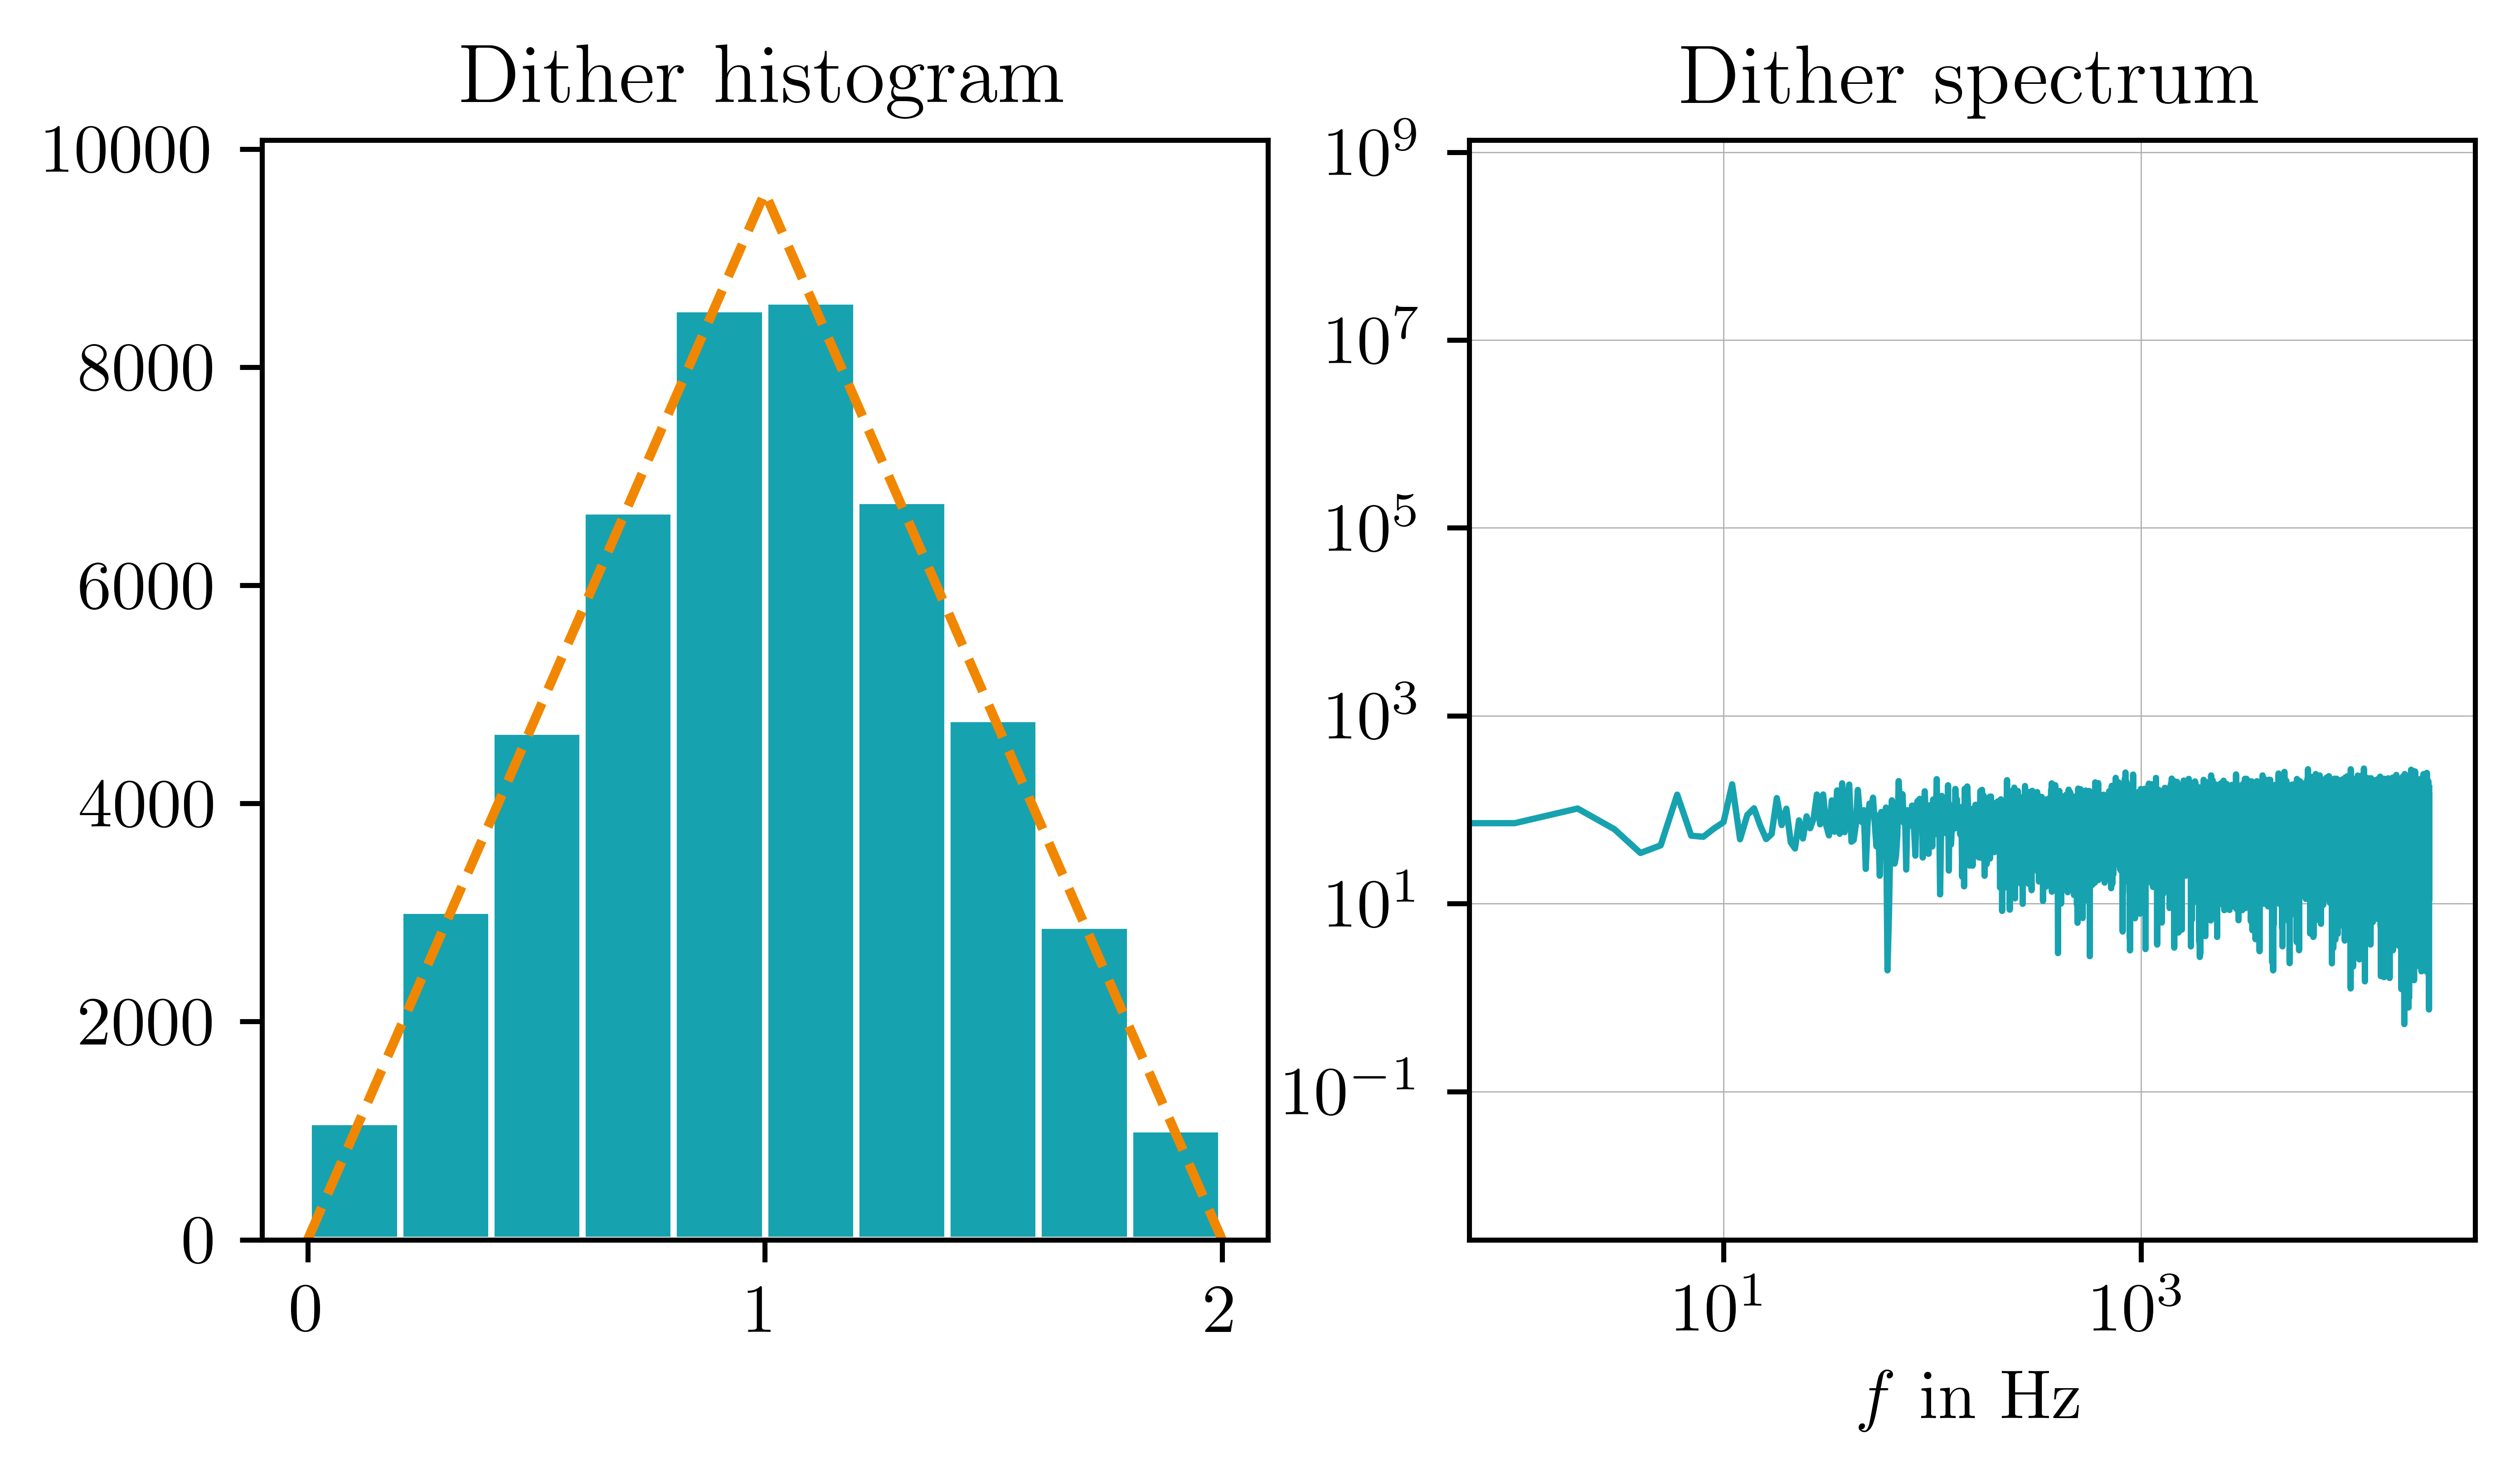
\includegraphics{./img/c63a50457e301fbac6f54c9be07067882f5cf91c.png}

\hypertarget{quantisierung}{%
\subsubsection{Quantisierung}\label{quantisierung}}

\begin{lstlisting}[language=Python]
# apply dither
signal_scaled_dither = signal_scaled - dither_scaled

# quantization using a quantizer function
delta = (2**(8))
quantized_signal = delta * np.floor((signal_scaled / delta) + (1/2))
quantized_signal_dither = delta * np.floor((signal_scaled_dither / delta) + (1/2))

plt.plot(np.abs(fft(quantized_signal_dither)[1:FS//2]), color="#13a538", lw=1)
plt.plot(np.abs(fft(quantized_signal)[1:FS//2]), color="#b2110e", lw=1)
plt.plot(np.abs(fft(signal_scaled)[1:FS//2]), color="#0085c8", lw=1)
plt.grid(which="both", linewidth=0.2)

plt.legend(["Dithered \& Quantized", "Quantized", "Original"], loc="lower left", fontsize="small")
plt.grid(which="both", linewidth=0.2)

plt.loglog()
plt.xlabel("$f$ in Hz")
plt.gca().set_ylim(ylim)

plt.show()
\end{lstlisting}

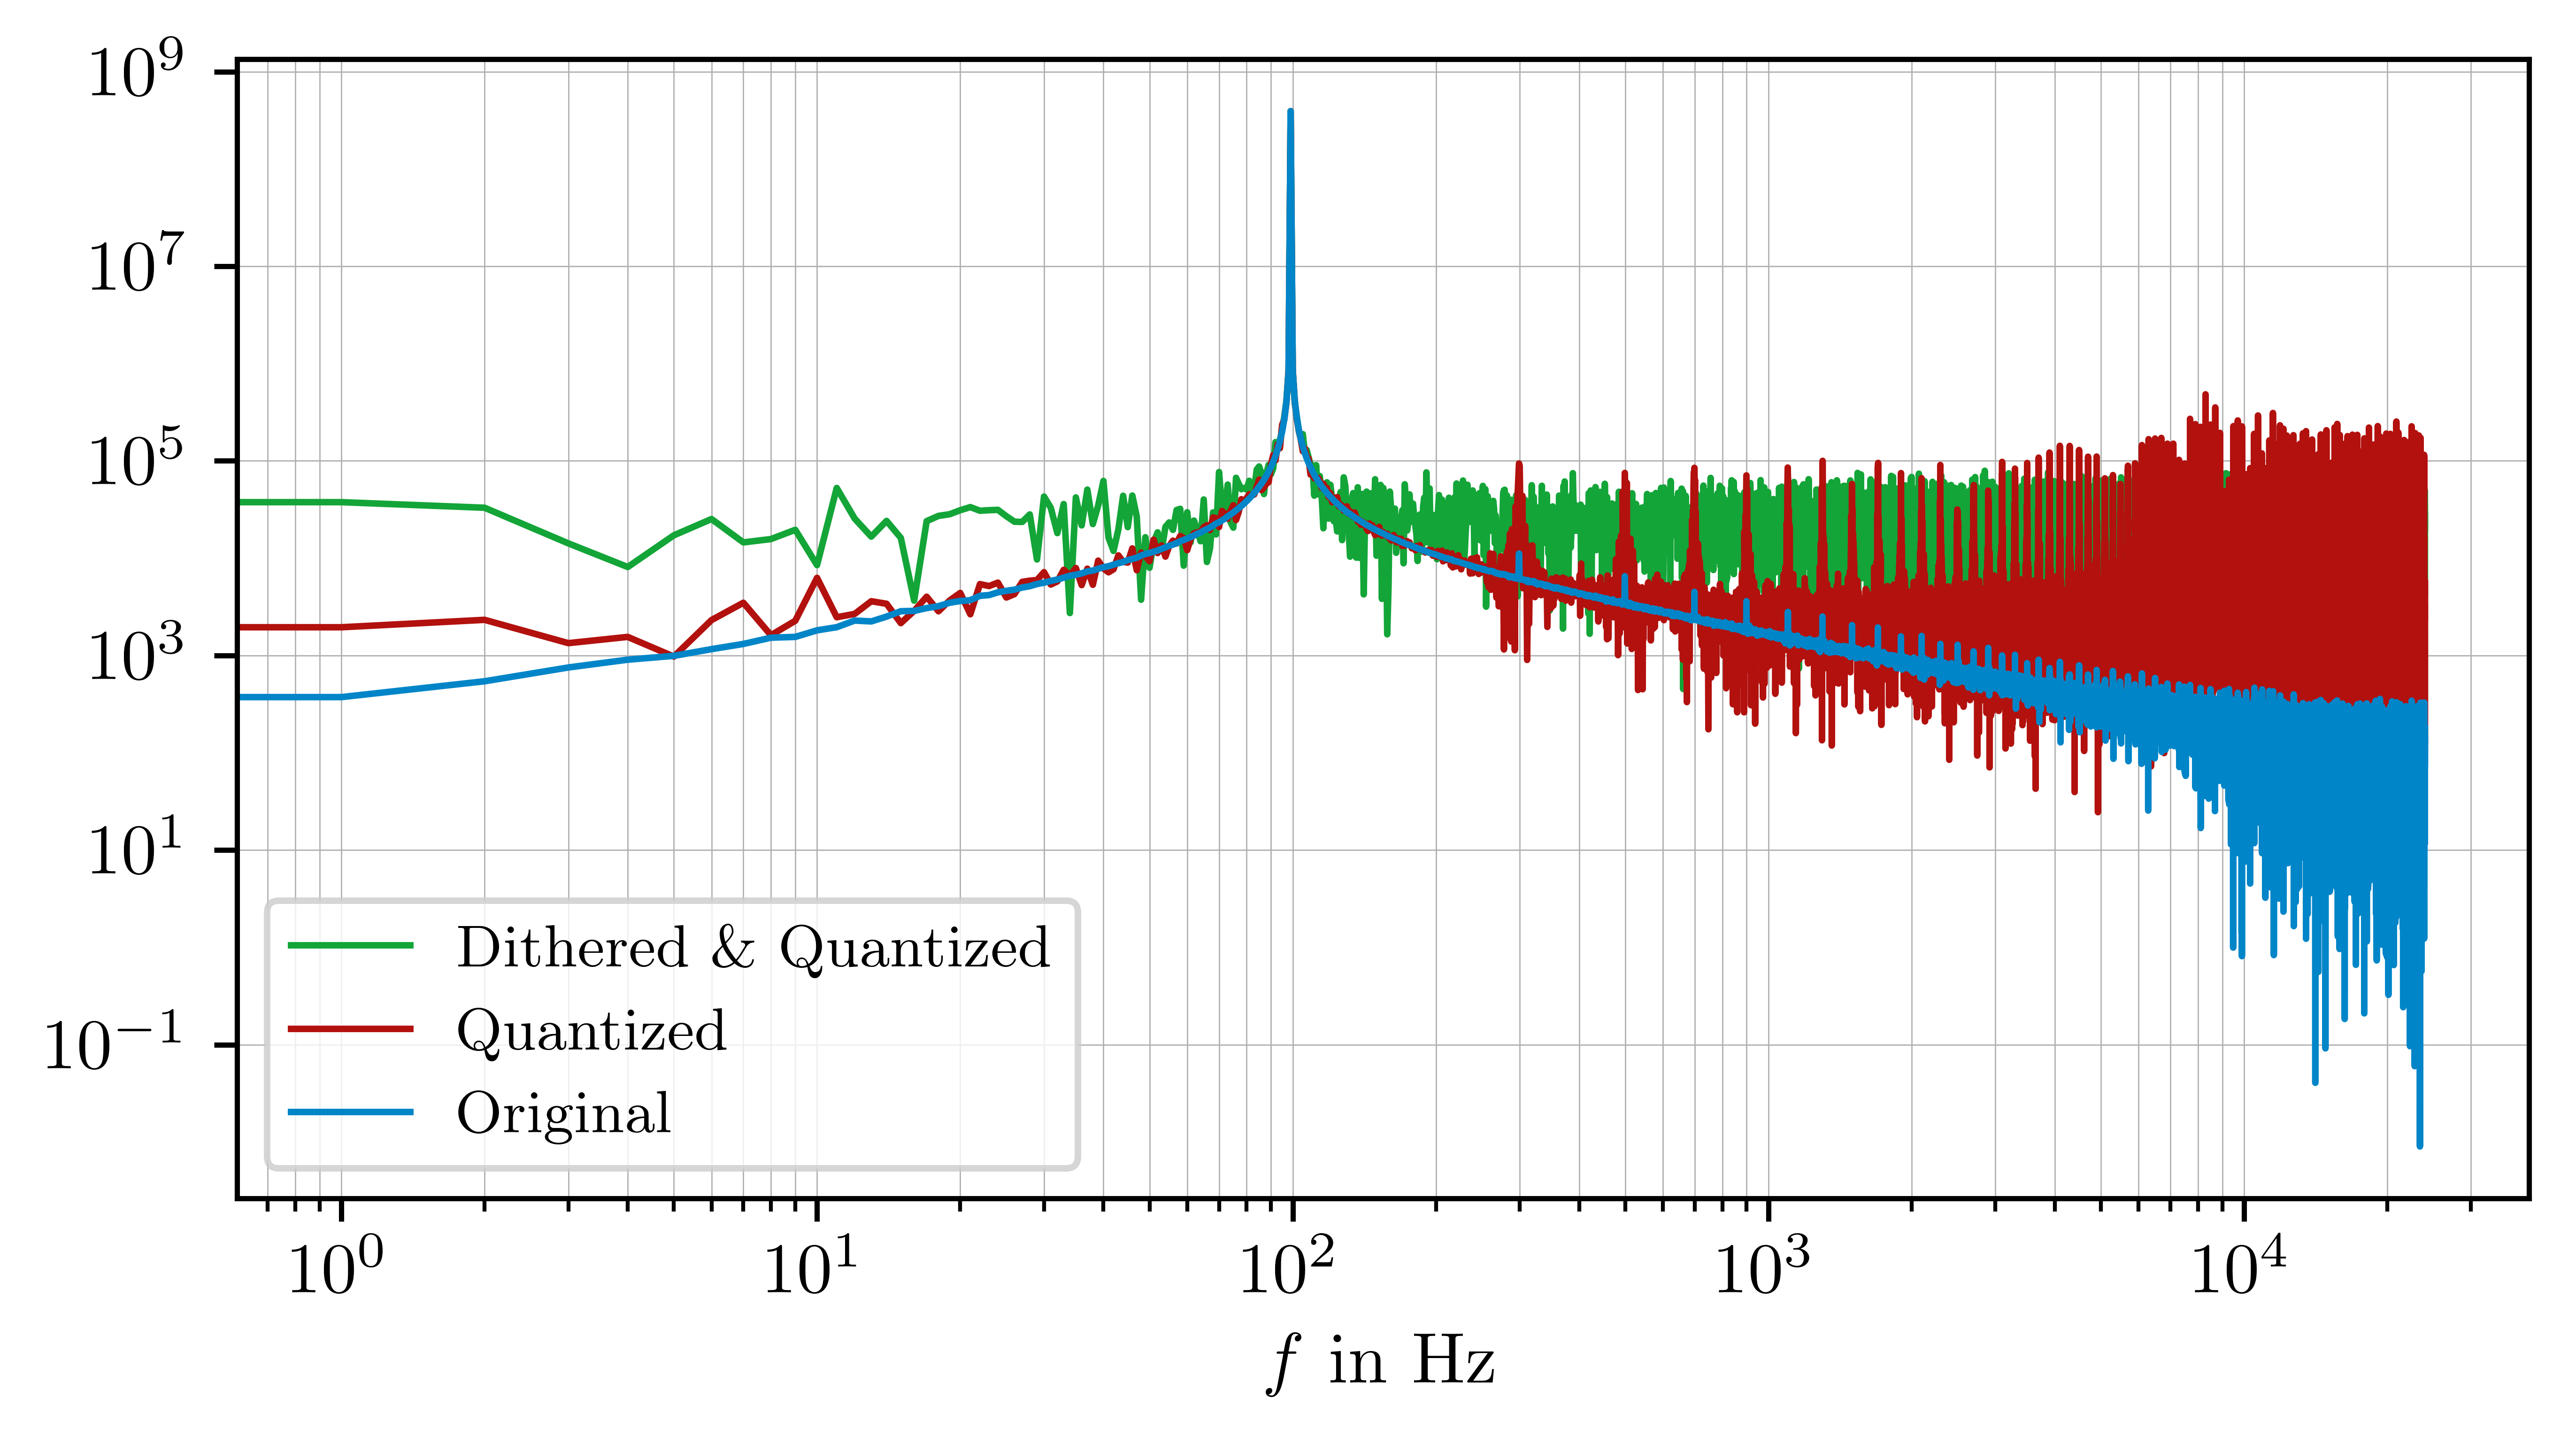
\includegraphics{./img/f7e4a300529452ae2941ee97f44efef8b6dfe4fd.png}

Dieses überzogene Beispiel demonstriert das Quantisierungsrauschen und
den Effekt des Dithers. Jedes Signal zeigt noch immer den Ton bei
\(100\) Herz. Das quantisierte Signal besitzt dazu einige harmonische
Übertöne im Vergleich zum originalen. Das Signal mit Dither hat keine
Übertöne, dafür jedoch ein wesentlich reduziertes \gls{snr}.

\hypertarget{rauschformungsfilter-ruxfcckkopplungsschleife}{%
\subsubsection{Rauschformungsfilter
Rückkopplungsschleife}\label{rauschformungsfilter-ruxfcckkopplungsschleife}}

Dieser Loop implementiert den gesamten Rauschformungsprozess.

\begin{lstlisting}[language=Python]
quantized_signal_noise_shaped = [0] * len(signal)
filter_buffer = [0] * len(kernel)
filtered_error = 0

# Noise shaping feedback loop
for n in range(len(signal)):
    sample = signal_scaled[n] - filtered_error
    dithered_sample = sample - dither_scaled[n]
    quantized_sample = delta * np.floor((dithered_sample / delta) + (1/2))

    error = quantized_sample - sample
    filter_buffer.append(error)
    filtered_error = 0

    # Convolution
    for k in range(len(kernel)):
        filtered_error = filtered_error + filter_buffer[n-k] * kernel[k]

    quantized_signal_noise_shaped[n] = (sample)
\end{lstlisting}

\begin{lstlisting}[language=Python]
plt.plot(np.abs(fft(quantized_signal_dither)[1:FS//2]), color="#13a538", lw=1)
plt.plot(np.abs(fft(quantized_signal_noise_shaped)[1:FS//2]), color="#59358c", lw=1)
plt.plot(np.abs(fft(signal_scaled)[1:FS//2]), color="#0085c8", lw=1)
plt.grid(which="both", linewidth=0.2)

plt.legend(["Dithered \& Quantized", "Noise-Shaped", "Original"], loc="lower left", fontsize="small")

plt.loglog()
plt.xlabel("$f$ in Hz")
plt.gca().set_ylim(ylim)

plt.show()
\end{lstlisting}

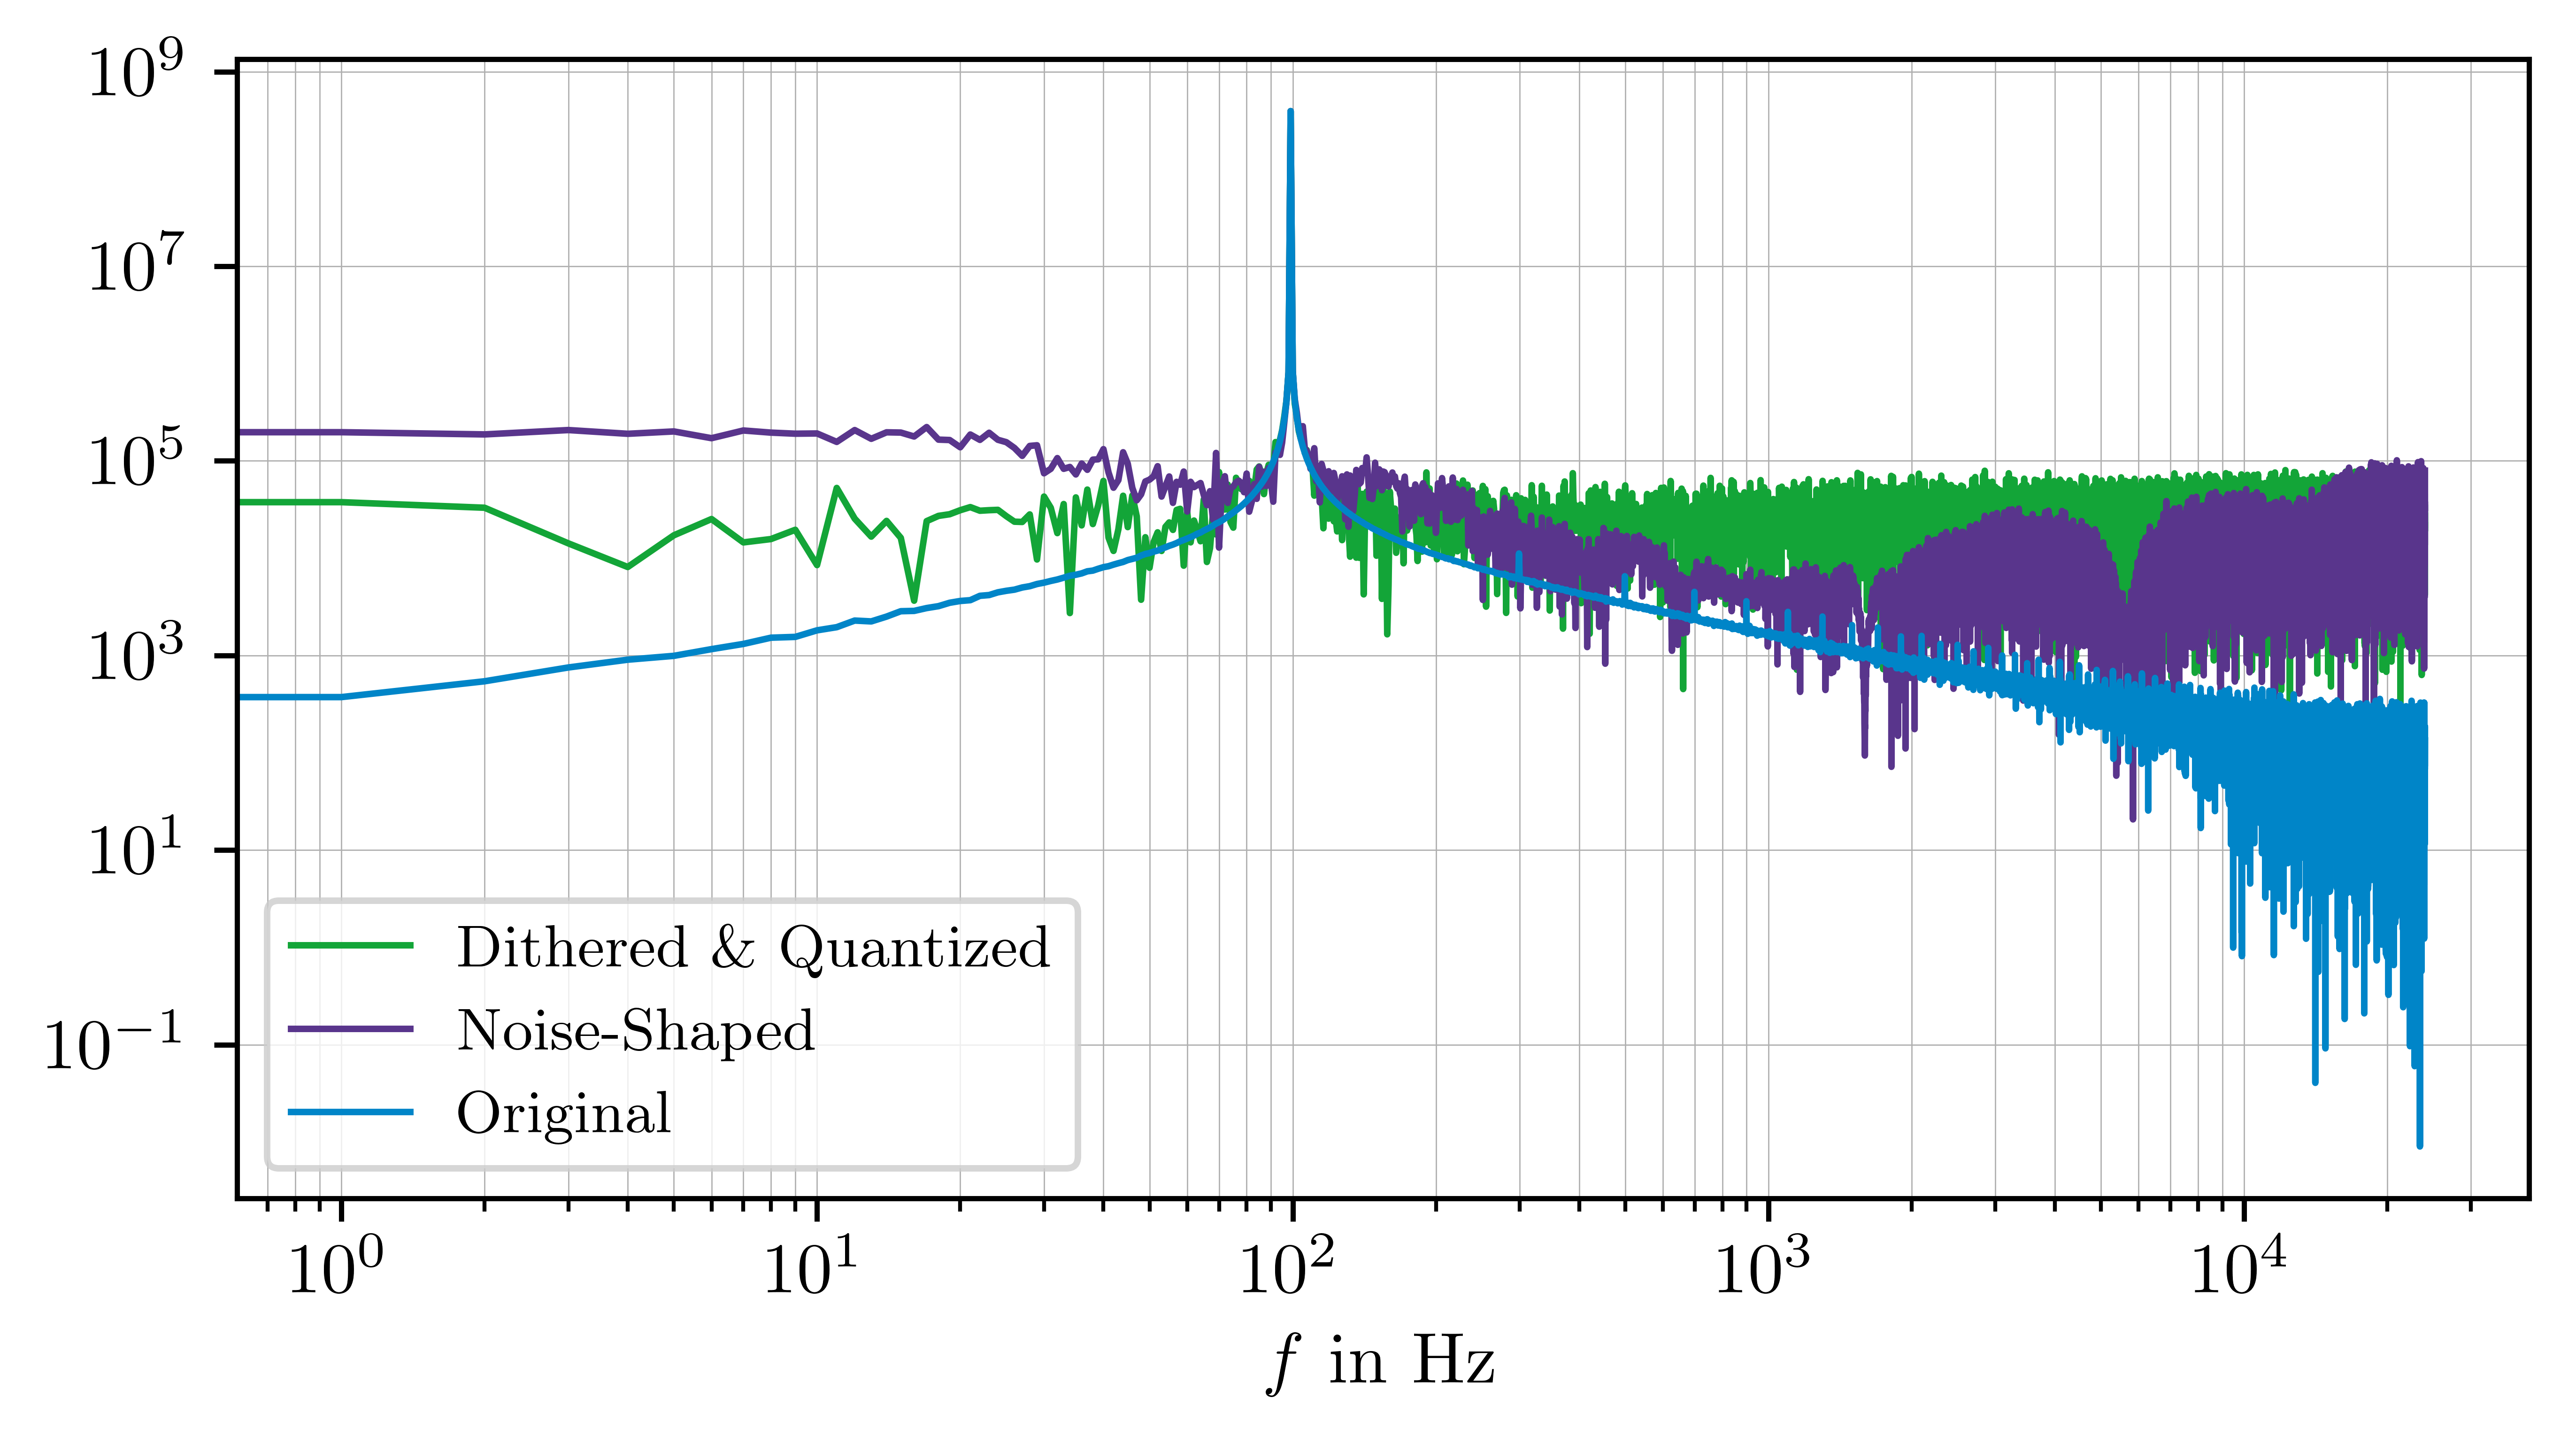
\includegraphics{./img/ae196e89b8edac3c7e803947e775a4f5c07fa49f.png}

In diesem Beispiel ist die spektrale Formung des Rauschens anschaulich
demonstriert. Der Effekt ist hier, wie schon mehrmals erwähnt, stark
dramatisiert. Das grundlegende Konzept ist jedoch auch in der realen
Implementation identisch.

Das geformte Rauschen nimmt die Form der Zielfunktion an. Es wird in
Summe keine Energie zugefügt oder entzogen. Der Rauschformungsfilter
funktioniert.

\hfill\(\blacksquare\)
